% All appendices, in one file. avi.tex pulls it in with % All appendices, in one file. avi.tex pulls it in with % All appendices, in one file. avi.tex pulls it in with % All appendices, in one file. avi.tex pulls it in with \input{appendix/appendix}; no preamble here.
% One big unnumbered section, "Appendix"; each part is a subsection lettered A, B, C, ...
% Add the next part as another \subsection{...}\label{app:...} below.
\section*{Appendix}\label{sec:appendix}
\addcontentsline{toc}{section}{Appendix}
\setcounter{subsection}{0}
\renewcommand{\thesubsection}{\Alph{subsection}}

\subsection{bench60}\label{app:bench60}

\begin{definition}[bench60, full rule]\label{def:bench60full}
Let $g_0=3$ and $g_{10}=574{,}959$ be the least and the largest value of $g$ on MS640 at budget $10^6$, and
let $\rho=(g_{10}/g_0)^{1/10}\approx3.37$. The \emph{difficulty class} $b\in\{0,\dots,9\}$ is the set of $P\in$ MS640 with
$g_0\rho^{b}\le g(P)<g_0\rho^{b+1}$ (class $9$ closed on the right). \textbf{bench60} takes $6$ presentations from every
difficulty class by the following rule.
\begin{enumerate}
  \item Over the whole subset, minimise the number of pairs of chosen presentations in the same $\Aut(\F_2)$-orbit.
  \item Subject to (1), sort the presentations of each difficulty class by path length, the number of S-moves in the solution GS-SUB finds; break ties by smaller $g$ first, then by line number in MS640.
  Take the $6$ presentations closest to $6$ evenly spaced positions of this sorted list, the first and the last
  position included.
  % This one needs more explaination
\end{enumerate}
\end{definition}

Figure~\ref{fig:bench60} shows where the $60$ rows lie in MS640.

\begin{center}
\begin{tabular}{rrrrr}
\toprule
class $b$ & range of $g$ & rows of MS640 & rows of bench60 & mean $g$ on bench60\\
\midrule
0 & $[3,\,11)$ & $317$ & $6$ & $6.3$\\
1 & $[11,\,35)$ & $89$ & $6$ & $17.7$\\
2 & $[35,\,116)$ & $63$ & $6$ & $74.3$\\
3 & $[116,\,390)$ & $60$ & $6$ & $261.7$\\
4 & $[390,\,1{,}314)$ & $31$ & $6$ & $691.2$\\
5 & $[1{,}314,\,4{,}433)$ & $26$ & $6$ & $1{,}746.8$\\
6 & $[4{,}433,\,14{,}959)$ & $28$ & $6$ & $9{,}869.2$\\
7 & $[14{,}959,\,50{,}482)$ & $14$ & $6$ & $19{,}596.3$\\
8 & $[50{,}482,\,170{,}367)$ & $6$ & $6$ & $66{,}530.7$\\
9 & $[170{,}367,\,574{,}959]$ & $6$ & $6$ & $353{,}647.7$\\
\midrule
all & & $640$ & $60$ & \\
\bottomrule
\end{tabular}
\end{center}

\begin{figure}[ht]
\centering
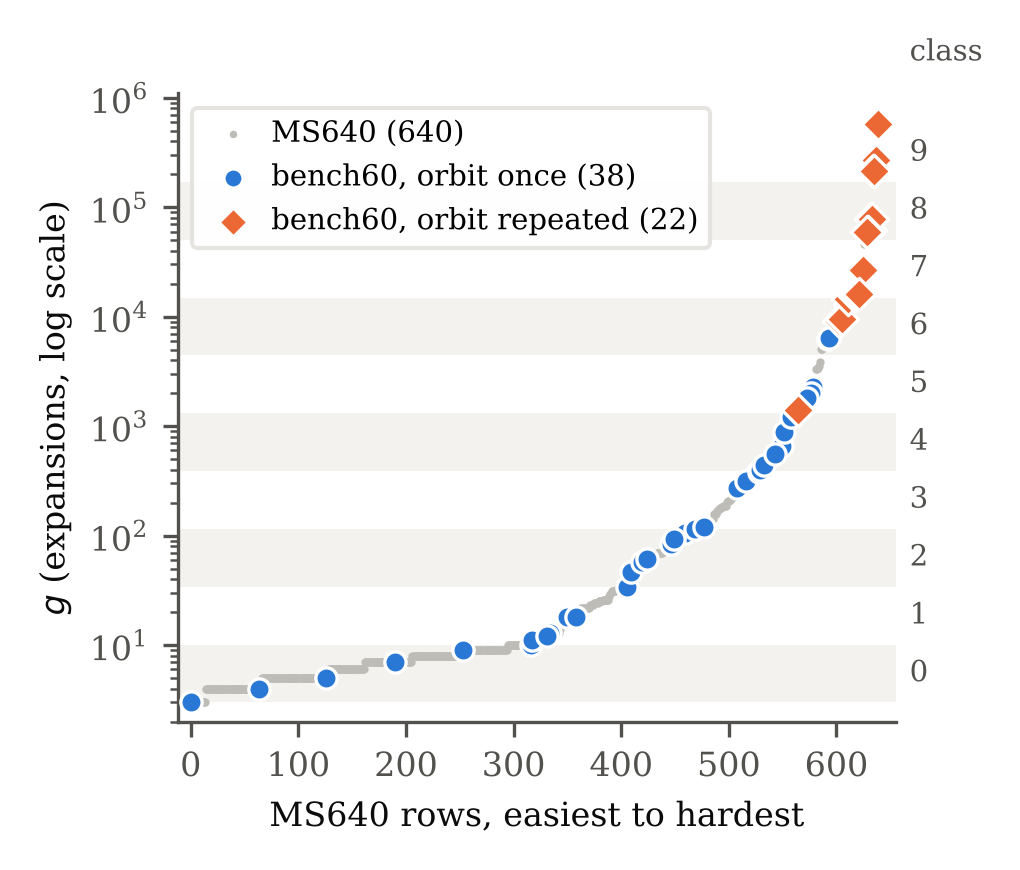
\includegraphics[width=0.49\textwidth]{figures/bench60_g.png}\hfill
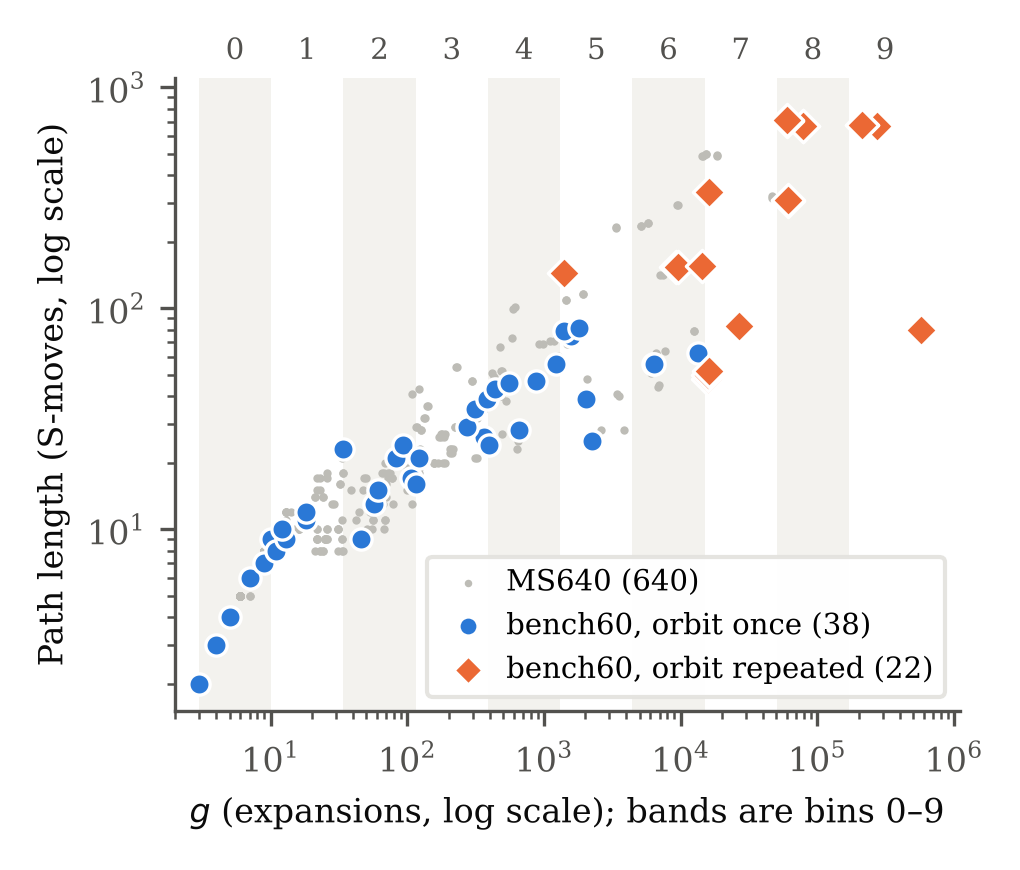
\includegraphics[width=0.49\textwidth]{figures/bench60_path.png}
\caption{bench60 inside MS640. Grey: all $640$ presentations; colour: the $60$ choices, six per difficulty class. Blue circles are choices whose
$\Aut(\F_2)$-orbit occurs once in bench60; diamonds are choices that share an orbit with another choice, which classes 7--9 force.
Left: $g$ against the rows sorted by $g$; the shaded bands are difficulty classes 0--9, each $3.37$ times the one below.
Right: the S-move length of a presentation against $g$.}
\label{fig:bench60}
\end{figure}

\subsection{ladder100}\label{app:ladder}

Each level of ladder100 (Definition~\ref{def:ladder}) contains $10$ presentations taken from AC19\_autmin and MS640;
Table~\ref{tab:ladder} gives the range of $g$ of each level. Here $g>10^7$ indicates that LENGTH fails within $10^7$
expansions, and $g_S$ denotes the number of expansions that $\SMK$ requires. At levels $1$--$6$ the presentations are
spread over the range of $g$ of the level, and at level $9$ over the range of $g_S$. Level $7$ takes the presentations
with the largest $g_S$, and level $8$ those with the largest $g$. Level $10$ consists of the presentations on which
$\SMK$ also fails within $10^7$ expansions.

Every presentation of ladder100 is AC-trivial. Those taken from MS640 are solved by LENGTH. For a presentation of
AC19\_autmin, the corresponding presentation of the extended AC19 data set is solved, and its S-moves are carried over to
the $\Aut(\F_2)$-minimal form.

\begin{table}[ht]
\centering
\begin{tabular}{rlrrrr}
\toprule
level & $g$ & from MS640 & mean $\lambda$ & mean $g$ & mean $g_S$\\
\midrule
1 & $<10^3$ & $5$ & $15.3$ & $214$ & $101$\\
2 & $10^3$--$10^4$ & $5$ & $19.9$ & $3{,}983$ & $707$\\
3 & $10^4$--$10^{4.5}$ & $5$ & $21.1$ & $17{,}612$ & $7{,}646$\\
4 & $10^{4.5}$--$10^5$ & $5$ & $21.5$ & $56{,}183$ & $9{,}780$\\
5 & $10^5$--$10^{5.5}$ & $4$ & $22.5$ & $235{,}756$ & $13{,}312$\\
6 & $10^{5.5}$--$10^6$ & $2$ & $19.4$ & $588{,}638$ & $4{,}693$\\
7 & $10^6$--$3\cdot10^6$ & $0$ & $20.2$ & $1{,}875{,}962$ & $424{,}977$\\
8 & $3\cdot10^6$--$10^7$ & $0$ & $18.8$ & $5{,}022{,}975$ & $113{,}309$\\
9 & $>10^7$ & $0$ & $21.0$ & -- & $340{,}650$\\
10$^{*}$ & $>10^7$ & $0$ & $18.3$ & -- & --\\
\bottomrule
\end{tabular}

\smallskip
{\small $^{*}$Only $9$ presentations fail for $\SMK$, so the tenth, \texttt{ac19\_12445}, is the next hardest one for
$\SMK$ from level $9$: it needs $1{,}297{,}772$ expansions.}
\caption{The levels of ladder100: the range of $g$, the number of the $10$ presentations taken from MS640 (the rest
are from AC19\_autmin), and the means of the starting total length $\lambda$, of $g$ and of $g_S$.}
\label{tab:ladder}
\end{table}

\subsection{Time per unit}\label{app:time}

An expansion performs different work in each method. LENGTH and $\SMK$ differ only in the priority they compute; the
hybrid additionally constructs the Nielsen images and runs the finishing checks; and a change of variables constructs
images of the state in place of S-move children. Equal budgets in units therefore constitute a fair comparison only
if a unit costs approximately the same in each method. To quantify the difference, one expansion of each method is
timed on the same states. For each test state, each method starts a fresh search, so that the heap holds only that
state, and performs one expansion: it removes the state, generates all of its children, discards those already
discovered, computes the priorities of the remainder and pushes them onto the heap. The test states are drawn at random
from the states that LENGTH and $\SMK$ expanded on MS640 with a budget of $10^4$ units, up to $60$ per range of total
length $\lambda$, and every method is timed on the same states. All methods run in pure Python (one core, Intel Xeon
$2.1$ GHz, best of five runs).
\begin{center}
\small
\begin{tabular}{lrrrrr}
\toprule
$\lambda$ & states & LENGTH & $\SMK$ & hybrid & CoV\\
\midrule
$\le10$ & $46$ & $0.12$ & $0.14$ & $0.28$ & $0.25$\\
$11$--$15$ & $60$ & $0.85$ & $1.05$ & $1.37$ & $3.24$\\
$16$--$20$ & $60$ & $1.61$ & $2.00$ & $3.03$ & $6.05$\\
$21$--$25$ & $60$ & $2.99$ & $3.41$ & $10.08$ & $11.23$\\
$\ge26$ & $60$ & $4.66$ & $6.00$ & $6.85$ & $16.47$\\
\midrule
mean & & $2.04$ & $2.52$ & $4.32$ & $7.45$\\
relative to LENGTH & & $1$ & $1.23$ & $2.11$ & $3.64$\\
\bottomrule
\end{tabular}

\smallskip
\footnotesize Time of one pop in ms, averaged over the states of the row. The mean row averages the five rows; the last row divides it by the LENGTH mean.
\end{center}
For example, one expansion of $\mathrm{AK}(3)$ ($\lambda=13$) takes $0.69$ ms for LENGTH, $0.87$ ms for $\SMK$,
$1.17$ ms for the hybrid and $2.61$ ms for the change of variables. A longer state has more children, so its expansion
costs more. An expansion of $\SMK$ differs from one of LENGTH only in its priority and costs $1.1$--$1.3$ times as much.
An expansion of the hybrid also constructs the four Nielsen images and runs the finishing checks, and costs $1.5$--$3.4$
times as much; its remaining units are single moves and cost less. Constructing the change-of-variables images of a
state costs $3.5$--$3.8$ expansions of LENGTH for $\lambda>10$. A unit of each method thus costs within a small factor
of one expansion of LENGTH, and equal budgets in units are comparable up to that factor.
; no preamble here.
% One big unnumbered section, "Appendix"; each part is a subsection lettered A, B, C, ...
% Add the next part as another \subsection{...}\label{app:...} below.
\section*{Appendix}\label{sec:appendix}
\addcontentsline{toc}{section}{Appendix}
\setcounter{subsection}{0}
\renewcommand{\thesubsection}{\Alph{subsection}}

\subsection{bench60}\label{app:bench60}

\begin{definition}[bench60, full rule]\label{def:bench60full}
Let $g_0=3$ and $g_{10}=574{,}959$ be the least and the largest value of $g$ on MS640 at budget $10^6$, and
let $\rho=(g_{10}/g_0)^{1/10}\approx3.37$. The \emph{difficulty class} $b\in\{0,\dots,9\}$ is the set of $P\in$ MS640 with
$g_0\rho^{b}\le g(P)<g_0\rho^{b+1}$ (class $9$ closed on the right). \textbf{bench60} takes $6$ presentations from every
difficulty class by the following rule.
\begin{enumerate}
  \item Over the whole subset, minimise the number of pairs of chosen presentations in the same $\Aut(\F_2)$-orbit.
  \item Subject to (1), sort the presentations of each difficulty class by path length, the number of S-moves in the solution GS-SUB finds; break ties by smaller $g$ first, then by line number in MS640.
  Take the $6$ presentations closest to $6$ evenly spaced positions of this sorted list, the first and the last
  position included.
  % This one needs more explaination
\end{enumerate}
\end{definition}

Figure~\ref{fig:bench60} shows where the $60$ rows lie in MS640.

\begin{center}
\begin{tabular}{rrrrr}
\toprule
class $b$ & range of $g$ & rows of MS640 & rows of bench60 & mean $g$ on bench60\\
\midrule
0 & $[3,\,11)$ & $317$ & $6$ & $6.3$\\
1 & $[11,\,35)$ & $89$ & $6$ & $17.7$\\
2 & $[35,\,116)$ & $63$ & $6$ & $74.3$\\
3 & $[116,\,390)$ & $60$ & $6$ & $261.7$\\
4 & $[390,\,1{,}314)$ & $31$ & $6$ & $691.2$\\
5 & $[1{,}314,\,4{,}433)$ & $26$ & $6$ & $1{,}746.8$\\
6 & $[4{,}433,\,14{,}959)$ & $28$ & $6$ & $9{,}869.2$\\
7 & $[14{,}959,\,50{,}482)$ & $14$ & $6$ & $19{,}596.3$\\
8 & $[50{,}482,\,170{,}367)$ & $6$ & $6$ & $66{,}530.7$\\
9 & $[170{,}367,\,574{,}959]$ & $6$ & $6$ & $353{,}647.7$\\
\midrule
all & & $640$ & $60$ & \\
\bottomrule
\end{tabular}
\end{center}

\begin{figure}[ht]
\centering
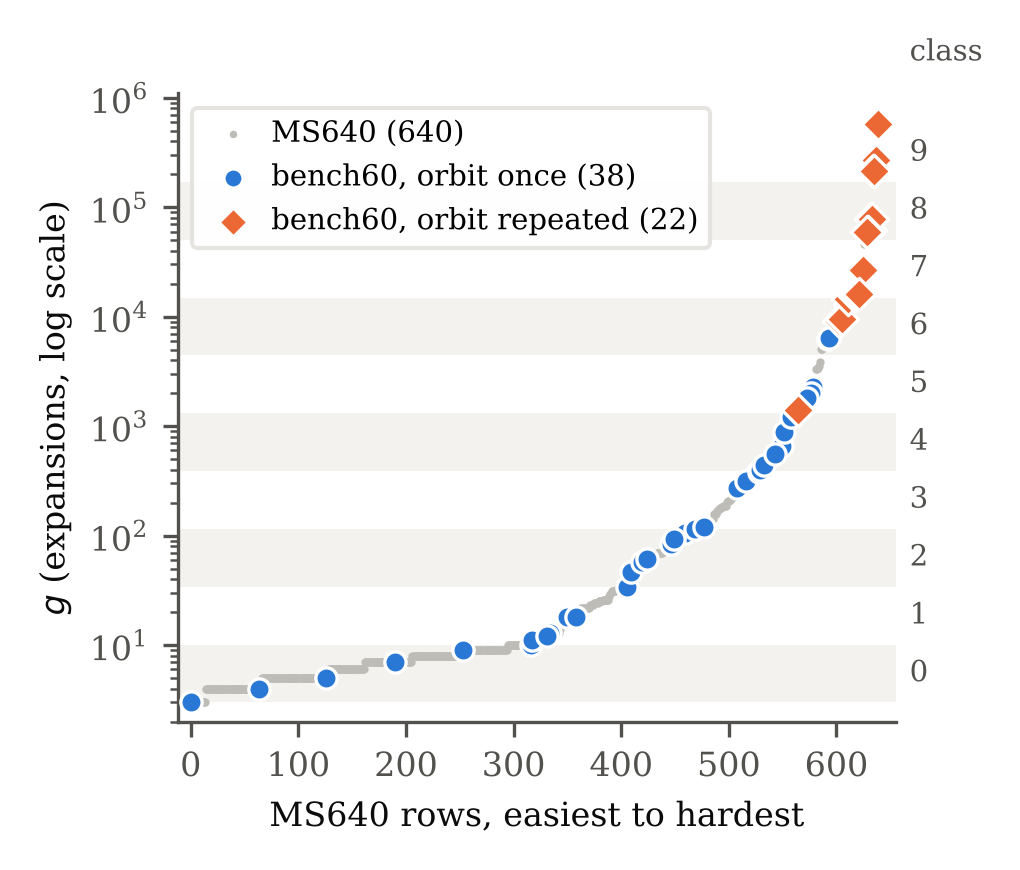
\includegraphics[width=0.49\textwidth]{figures/bench60_g.png}\hfill
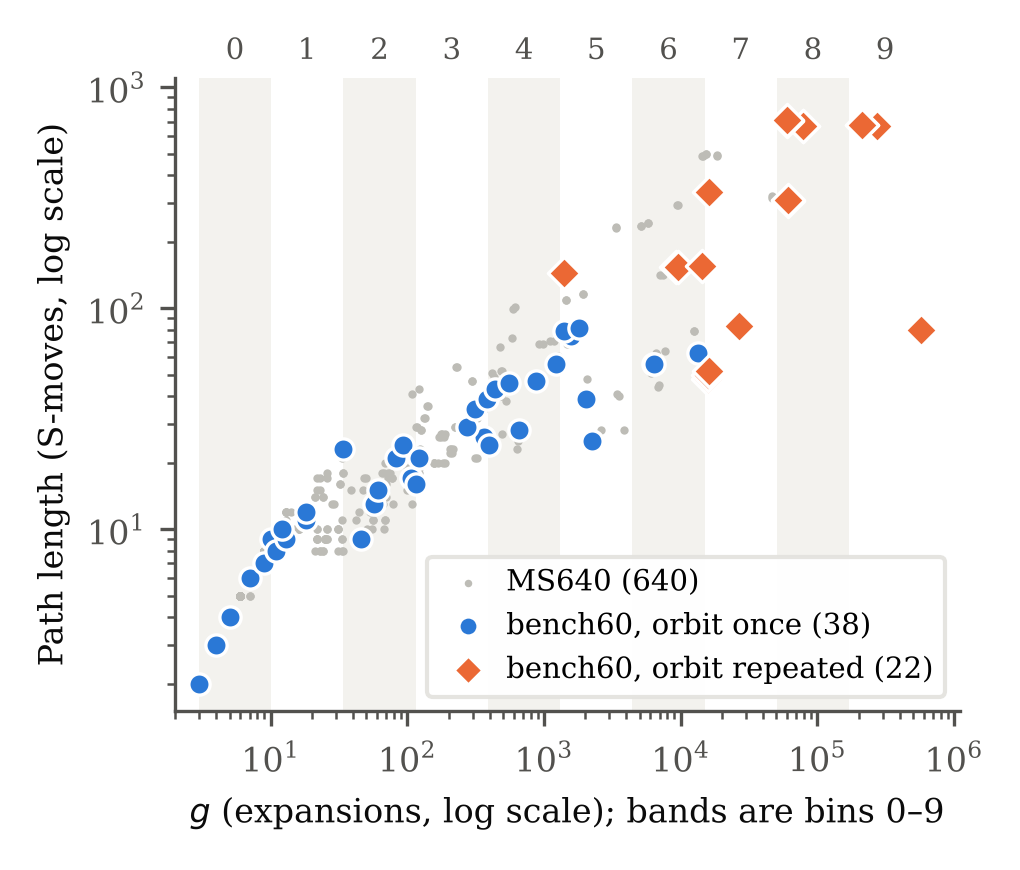
\includegraphics[width=0.49\textwidth]{figures/bench60_path.png}
\caption{bench60 inside MS640. Grey: all $640$ presentations; colour: the $60$ choices, six per difficulty class. Blue circles are choices whose
$\Aut(\F_2)$-orbit occurs once in bench60; diamonds are choices that share an orbit with another choice, which classes 7--9 force.
Left: $g$ against the rows sorted by $g$; the shaded bands are difficulty classes 0--9, each $3.37$ times the one below.
Right: the S-move length of a presentation against $g$.}
\label{fig:bench60}
\end{figure}

\subsection{ladder100}\label{app:ladder}

Each level of ladder100 (Definition~\ref{def:ladder}) contains $10$ presentations taken from AC19\_autmin and MS640;
Table~\ref{tab:ladder} gives the range of $g$ of each level. Here $g>10^7$ indicates that LENGTH fails within $10^7$
expansions, and $g_S$ denotes the number of expansions that $\SMK$ requires. At levels $1$--$6$ the presentations are
spread over the range of $g$ of the level, and at level $9$ over the range of $g_S$. Level $7$ takes the presentations
with the largest $g_S$, and level $8$ those with the largest $g$. Level $10$ consists of the presentations on which
$\SMK$ also fails within $10^7$ expansions.

Every presentation of ladder100 is AC-trivial. Those taken from MS640 are solved by LENGTH. For a presentation of
AC19\_autmin, the corresponding presentation of the extended AC19 data set is solved, and its S-moves are carried over to
the $\Aut(\F_2)$-minimal form.

\begin{table}[ht]
\centering
\begin{tabular}{rlrrrr}
\toprule
level & $g$ & from MS640 & mean $\lambda$ & mean $g$ & mean $g_S$\\
\midrule
1 & $<10^3$ & $5$ & $15.3$ & $214$ & $101$\\
2 & $10^3$--$10^4$ & $5$ & $19.9$ & $3{,}983$ & $707$\\
3 & $10^4$--$10^{4.5}$ & $5$ & $21.1$ & $17{,}612$ & $7{,}646$\\
4 & $10^{4.5}$--$10^5$ & $5$ & $21.5$ & $56{,}183$ & $9{,}780$\\
5 & $10^5$--$10^{5.5}$ & $4$ & $22.5$ & $235{,}756$ & $13{,}312$\\
6 & $10^{5.5}$--$10^6$ & $2$ & $19.4$ & $588{,}638$ & $4{,}693$\\
7 & $10^6$--$3\cdot10^6$ & $0$ & $20.2$ & $1{,}875{,}962$ & $424{,}977$\\
8 & $3\cdot10^6$--$10^7$ & $0$ & $18.8$ & $5{,}022{,}975$ & $113{,}309$\\
9 & $>10^7$ & $0$ & $21.0$ & -- & $340{,}650$\\
10$^{*}$ & $>10^7$ & $0$ & $18.3$ & -- & --\\
\bottomrule
\end{tabular}

\smallskip
{\small $^{*}$Only $9$ presentations fail for $\SMK$, so the tenth, \texttt{ac19\_12445}, is the next hardest one for
$\SMK$ from level $9$: it needs $1{,}297{,}772$ expansions.}
\caption{The levels of ladder100: the range of $g$, the number of the $10$ presentations taken from MS640 (the rest
are from AC19\_autmin), and the means of the starting total length $\lambda$, of $g$ and of $g_S$.}
\label{tab:ladder}
\end{table}

\subsection{Time per unit}\label{app:time}

An expansion performs different work in each method. LENGTH and $\SMK$ differ only in the priority they compute; the
hybrid additionally constructs the Nielsen images and runs the finishing checks; and a change of variables constructs
images of the state in place of S-move children. Equal budgets in units therefore constitute a fair comparison only
if a unit costs approximately the same in each method. To quantify the difference, one expansion of each method is
timed on the same states. For each test state, each method starts a fresh search, so that the heap holds only that
state, and performs one expansion: it removes the state, generates all of its children, discards those already
discovered, computes the priorities of the remainder and pushes them onto the heap. The test states are drawn at random
from the states that LENGTH and $\SMK$ expanded on MS640 with a budget of $10^4$ units, up to $60$ per range of total
length $\lambda$, and every method is timed on the same states. All methods run in pure Python (one core, Intel Xeon
$2.1$ GHz, best of five runs).
\begin{center}
\small
\begin{tabular}{lrrrrr}
\toprule
$\lambda$ & states & LENGTH & $\SMK$ & hybrid & CoV\\
\midrule
$\le10$ & $46$ & $0.12$ & $0.14$ & $0.28$ & $0.25$\\
$11$--$15$ & $60$ & $0.85$ & $1.05$ & $1.37$ & $3.24$\\
$16$--$20$ & $60$ & $1.61$ & $2.00$ & $3.03$ & $6.05$\\
$21$--$25$ & $60$ & $2.99$ & $3.41$ & $10.08$ & $11.23$\\
$\ge26$ & $60$ & $4.66$ & $6.00$ & $6.85$ & $16.47$\\
\midrule
mean & & $2.04$ & $2.52$ & $4.32$ & $7.45$\\
relative to LENGTH & & $1$ & $1.23$ & $2.11$ & $3.64$\\
\bottomrule
\end{tabular}

\smallskip
\footnotesize Time of one pop in ms, averaged over the states of the row. The mean row averages the five rows; the last row divides it by the LENGTH mean.
\end{center}
For example, one expansion of $\mathrm{AK}(3)$ ($\lambda=13$) takes $0.69$ ms for LENGTH, $0.87$ ms for $\SMK$,
$1.17$ ms for the hybrid and $2.61$ ms for the change of variables. A longer state has more children, so its expansion
costs more. An expansion of $\SMK$ differs from one of LENGTH only in its priority and costs $1.1$--$1.3$ times as much.
An expansion of the hybrid also constructs the four Nielsen images and runs the finishing checks, and costs $1.5$--$3.4$
times as much; its remaining units are single moves and cost less. Constructing the change-of-variables images of a
state costs $3.5$--$3.8$ expansions of LENGTH for $\lambda>10$. A unit of each method thus costs within a small factor
of one expansion of LENGTH, and equal budgets in units are comparable up to that factor.
; no preamble here.
% One big unnumbered section, "Appendix"; each part is a subsection lettered A, B, C, ...
% Add the next part as another \subsection{...}\label{app:...} below.
\section*{Appendix}\label{sec:appendix}
\addcontentsline{toc}{section}{Appendix}
\setcounter{subsection}{0}
\renewcommand{\thesubsection}{\Alph{subsection}}

\subsection{bench60}\label{app:bench60}

\begin{definition}[bench60, full rule]\label{def:bench60full}
Let $g_0=3$ and $g_{10}=574{,}959$ be the least and the largest value of $g$ on MS640 at budget $10^6$, and
let $\rho=(g_{10}/g_0)^{1/10}\approx3.37$. The \emph{difficulty class} $b\in\{0,\dots,9\}$ is the set of $P\in$ MS640 with
$g_0\rho^{b}\le g(P)<g_0\rho^{b+1}$ (class $9$ closed on the right). \textbf{bench60} takes $6$ presentations from every
difficulty class by the following rule.
\begin{enumerate}
  \item Over the whole subset, minimise the number of pairs of chosen presentations in the same $\Aut(\F_2)$-orbit.
  \item Subject to (1), sort the presentations of each difficulty class by path length, the number of S-moves in the solution GS-SUB finds; break ties by smaller $g$ first, then by line number in MS640.
  Take the $6$ presentations closest to $6$ evenly spaced positions of this sorted list, the first and the last
  position included.
  % This one needs more explaination
\end{enumerate}
\end{definition}

Figure~\ref{fig:bench60} shows where the $60$ rows lie in MS640.

\begin{center}
\begin{tabular}{rrrrr}
\toprule
class $b$ & range of $g$ & rows of MS640 & rows of bench60 & mean $g$ on bench60\\
\midrule
0 & $[3,\,11)$ & $317$ & $6$ & $6.3$\\
1 & $[11,\,35)$ & $89$ & $6$ & $17.7$\\
2 & $[35,\,116)$ & $63$ & $6$ & $74.3$\\
3 & $[116,\,390)$ & $60$ & $6$ & $261.7$\\
4 & $[390,\,1{,}314)$ & $31$ & $6$ & $691.2$\\
5 & $[1{,}314,\,4{,}433)$ & $26$ & $6$ & $1{,}746.8$\\
6 & $[4{,}433,\,14{,}959)$ & $28$ & $6$ & $9{,}869.2$\\
7 & $[14{,}959,\,50{,}482)$ & $14$ & $6$ & $19{,}596.3$\\
8 & $[50{,}482,\,170{,}367)$ & $6$ & $6$ & $66{,}530.7$\\
9 & $[170{,}367,\,574{,}959]$ & $6$ & $6$ & $353{,}647.7$\\
\midrule
all & & $640$ & $60$ & \\
\bottomrule
\end{tabular}
\end{center}

\begin{figure}[ht]
\centering
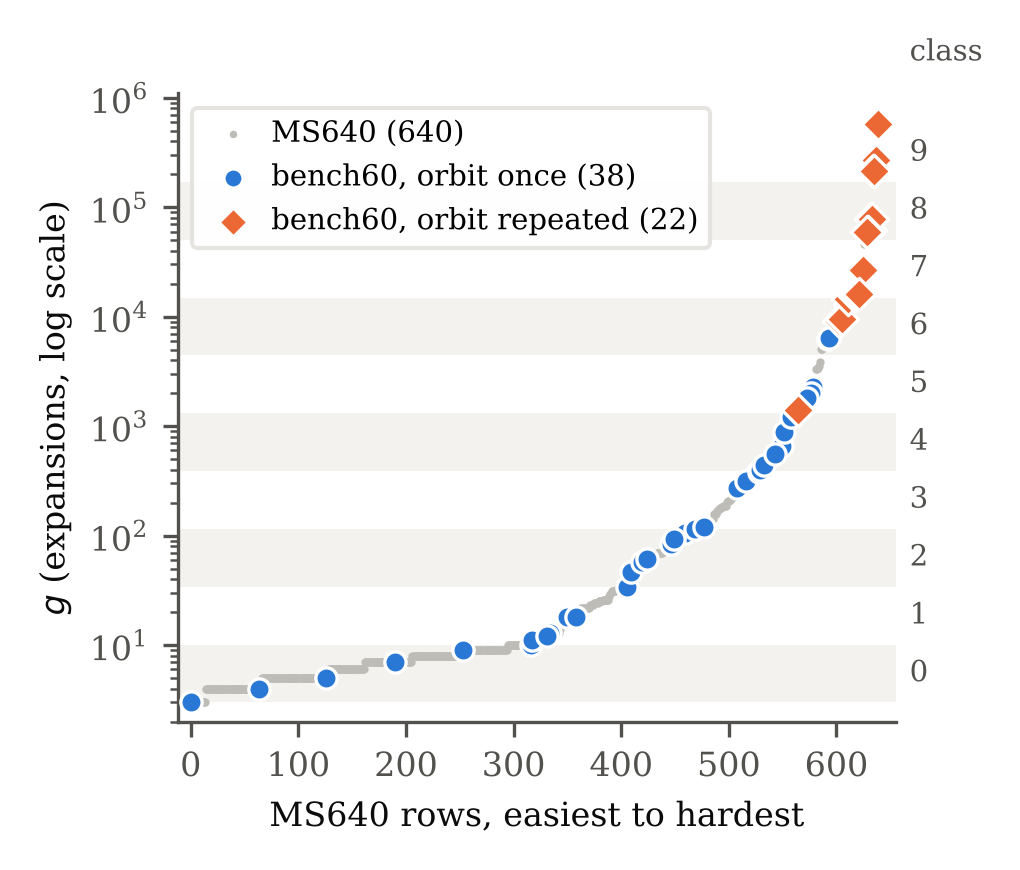
\includegraphics[width=0.49\textwidth]{figures/bench60_g.png}\hfill
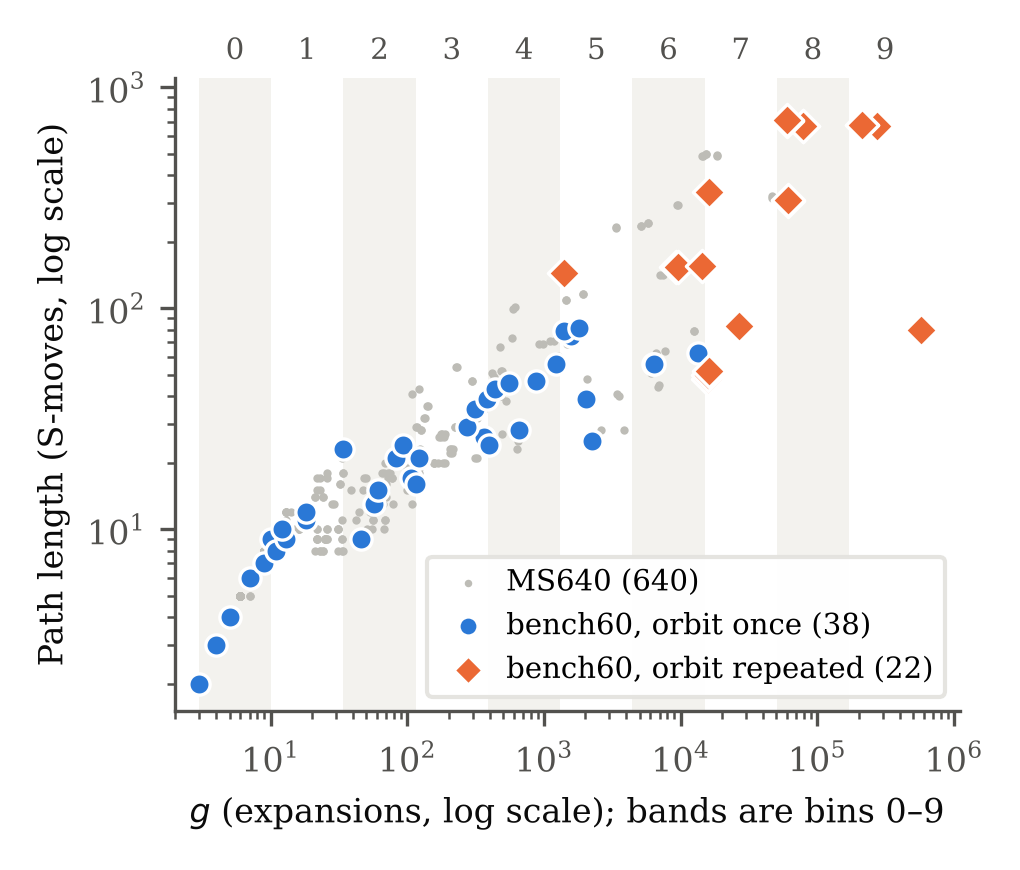
\includegraphics[width=0.49\textwidth]{figures/bench60_path.png}
\caption{bench60 inside MS640. Grey: all $640$ presentations; colour: the $60$ choices, six per difficulty class. Blue circles are choices whose
$\Aut(\F_2)$-orbit occurs once in bench60; diamonds are choices that share an orbit with another choice, which classes 7--9 force.
Left: $g$ against the rows sorted by $g$; the shaded bands are difficulty classes 0--9, each $3.37$ times the one below.
Right: the S-move length of a presentation against $g$.}
\label{fig:bench60}
\end{figure}

\subsection{ladder100}\label{app:ladder}

Each level of ladder100 (Definition~\ref{def:ladder}) contains $10$ presentations taken from AC19\_autmin and MS640;
Table~\ref{tab:ladder} gives the range of $g$ of each level. Here $g>10^7$ indicates that LENGTH fails within $10^7$
expansions, and $g_S$ denotes the number of expansions that $\SMK$ requires. At levels $1$--$6$ the presentations are
spread over the range of $g$ of the level, and at level $9$ over the range of $g_S$. Level $7$ takes the presentations
with the largest $g_S$, and level $8$ those with the largest $g$. Level $10$ consists of the presentations on which
$\SMK$ also fails within $10^7$ expansions.

Every presentation of ladder100 is AC-trivial. Those taken from MS640 are solved by LENGTH. For a presentation of
AC19\_autmin, the corresponding presentation of the extended AC19 data set is solved, and its S-moves are carried over to
the $\Aut(\F_2)$-minimal form.

\begin{table}[ht]
\centering
\begin{tabular}{rlrrrr}
\toprule
level & $g$ & from MS640 & mean $\lambda$ & mean $g$ & mean $g_S$\\
\midrule
1 & $<10^3$ & $5$ & $15.3$ & $214$ & $101$\\
2 & $10^3$--$10^4$ & $5$ & $19.9$ & $3{,}983$ & $707$\\
3 & $10^4$--$10^{4.5}$ & $5$ & $21.1$ & $17{,}612$ & $7{,}646$\\
4 & $10^{4.5}$--$10^5$ & $5$ & $21.5$ & $56{,}183$ & $9{,}780$\\
5 & $10^5$--$10^{5.5}$ & $4$ & $22.5$ & $235{,}756$ & $13{,}312$\\
6 & $10^{5.5}$--$10^6$ & $2$ & $19.4$ & $588{,}638$ & $4{,}693$\\
7 & $10^6$--$3\cdot10^6$ & $0$ & $20.2$ & $1{,}875{,}962$ & $424{,}977$\\
8 & $3\cdot10^6$--$10^7$ & $0$ & $18.8$ & $5{,}022{,}975$ & $113{,}309$\\
9 & $>10^7$ & $0$ & $21.0$ & -- & $340{,}650$\\
10$^{*}$ & $>10^7$ & $0$ & $18.3$ & -- & --\\
\bottomrule
\end{tabular}

\smallskip
{\small $^{*}$Only $9$ presentations fail for $\SMK$, so the tenth, \texttt{ac19\_12445}, is the next hardest one for
$\SMK$ from level $9$: it needs $1{,}297{,}772$ expansions.}
\caption{The levels of ladder100: the range of $g$, the number of the $10$ presentations taken from MS640 (the rest
are from AC19\_autmin), and the means of the starting total length $\lambda$, of $g$ and of $g_S$.}
\label{tab:ladder}
\end{table}

\subsection{Time per unit}\label{app:time}

An expansion performs different work in each method. LENGTH and $\SMK$ differ only in the priority they compute; the
hybrid additionally constructs the Nielsen images and runs the finishing checks; and a change of variables constructs
images of the state in place of S-move children. Equal budgets in units therefore constitute a fair comparison only
if a unit costs approximately the same in each method. To quantify the difference, one expansion of each method is
timed on the same states. For each test state, each method starts a fresh search, so that the heap holds only that
state, and performs one expansion: it removes the state, generates all of its children, discards those already
discovered, computes the priorities of the remainder and pushes them onto the heap. The test states are drawn at random
from the states that LENGTH and $\SMK$ expanded on MS640 with a budget of $10^4$ units, up to $60$ per range of total
length $\lambda$, and every method is timed on the same states. All methods run in pure Python (one core, Intel Xeon
$2.1$ GHz, best of five runs).
\begin{center}
\small
\begin{tabular}{lrrrrr}
\toprule
$\lambda$ & states & LENGTH & $\SMK$ & hybrid & CoV\\
\midrule
$\le10$ & $46$ & $0.12$ & $0.14$ & $0.28$ & $0.25$\\
$11$--$15$ & $60$ & $0.85$ & $1.05$ & $1.37$ & $3.24$\\
$16$--$20$ & $60$ & $1.61$ & $2.00$ & $3.03$ & $6.05$\\
$21$--$25$ & $60$ & $2.99$ & $3.41$ & $10.08$ & $11.23$\\
$\ge26$ & $60$ & $4.66$ & $6.00$ & $6.85$ & $16.47$\\
\midrule
mean & & $2.04$ & $2.52$ & $4.32$ & $7.45$\\
relative to LENGTH & & $1$ & $1.23$ & $2.11$ & $3.64$\\
\bottomrule
\end{tabular}

\smallskip
\footnotesize Time of one pop in ms, averaged over the states of the row. The mean row averages the five rows; the last row divides it by the LENGTH mean.
\end{center}
For example, one expansion of $\mathrm{AK}(3)$ ($\lambda=13$) takes $0.69$ ms for LENGTH, $0.87$ ms for $\SMK$,
$1.17$ ms for the hybrid and $2.61$ ms for the change of variables. A longer state has more children, so its expansion
costs more. An expansion of $\SMK$ differs from one of LENGTH only in its priority and costs $1.1$--$1.3$ times as much.
An expansion of the hybrid also constructs the four Nielsen images and runs the finishing checks, and costs $1.5$--$3.4$
times as much; its remaining units are single moves and cost less. Constructing the change-of-variables images of a
state costs $3.5$--$3.8$ expansions of LENGTH for $\lambda>10$. A unit of each method thus costs within a small factor
of one expansion of LENGTH, and equal budgets in units are comparable up to that factor.
; no preamble here.
% One big unnumbered section, "Appendix"; each part is a subsection lettered A, B, C, ...
% Add the next part as another \subsection{...}\label{app:...} below.
\section*{Appendix}\label{sec:appendix}
\addcontentsline{toc}{section}{Appendix}
\setcounter{subsection}{0}
\renewcommand{\thesubsection}{\Alph{subsection}}

\subsection{bench60}\label{app:bench60}

\begin{definition}[bench60, full rule]\label{def:bench60full}
Let $g_0=3$ and $g_{10}=574{,}959$ be the least and the largest value of $g$ on MS640 at budget $10^6$, and
let $\rho=(g_{10}/g_0)^{1/10}\approx3.37$. The \emph{difficulty class} $b\in\{0,\dots,9\}$ is the set of $P\in$ MS640 with
$g_0\rho^{b}\le g(P)<g_0\rho^{b+1}$ (class $9$ closed on the right). \textbf{bench60} takes $6$ presentations from every
difficulty class by the following rule.
\begin{enumerate}
  \item Over the whole subset, minimise the number of pairs of chosen presentations in the same $\Aut(\F_2)$-orbit.
  \item Subject to (1), sort the presentations of each difficulty class by path length, the number of S-moves in the solution GS-SUB finds; break ties by smaller $g$ first, then by line number in MS640.
  Take the $6$ presentations closest to $6$ evenly spaced positions of this sorted list, the first and the last
  position included.
  % This one needs more explaination
\end{enumerate}
\end{definition}

Figure~\ref{fig:bench60} shows where the $60$ rows lie in MS640.

\begin{center}
\begin{tabular}{rrrrr}
\toprule
class $b$ & range of $g$ & rows of MS640 & rows of bench60 & mean $g$ on bench60\\
\midrule
0 & $[3,\,11)$ & $317$ & $6$ & $6.3$\\
1 & $[11,\,35)$ & $89$ & $6$ & $17.7$\\
2 & $[35,\,116)$ & $63$ & $6$ & $74.3$\\
3 & $[116,\,390)$ & $60$ & $6$ & $261.7$\\
4 & $[390,\,1{,}314)$ & $31$ & $6$ & $691.2$\\
5 & $[1{,}314,\,4{,}433)$ & $26$ & $6$ & $1{,}746.8$\\
6 & $[4{,}433,\,14{,}959)$ & $28$ & $6$ & $9{,}869.2$\\
7 & $[14{,}959,\,50{,}482)$ & $14$ & $6$ & $19{,}596.3$\\
8 & $[50{,}482,\,170{,}367)$ & $6$ & $6$ & $66{,}530.7$\\
9 & $[170{,}367,\,574{,}959]$ & $6$ & $6$ & $353{,}647.7$\\
\midrule
all & & $640$ & $60$ & \\
\bottomrule
\end{tabular}
\end{center}

\begin{figure}[ht]
\centering
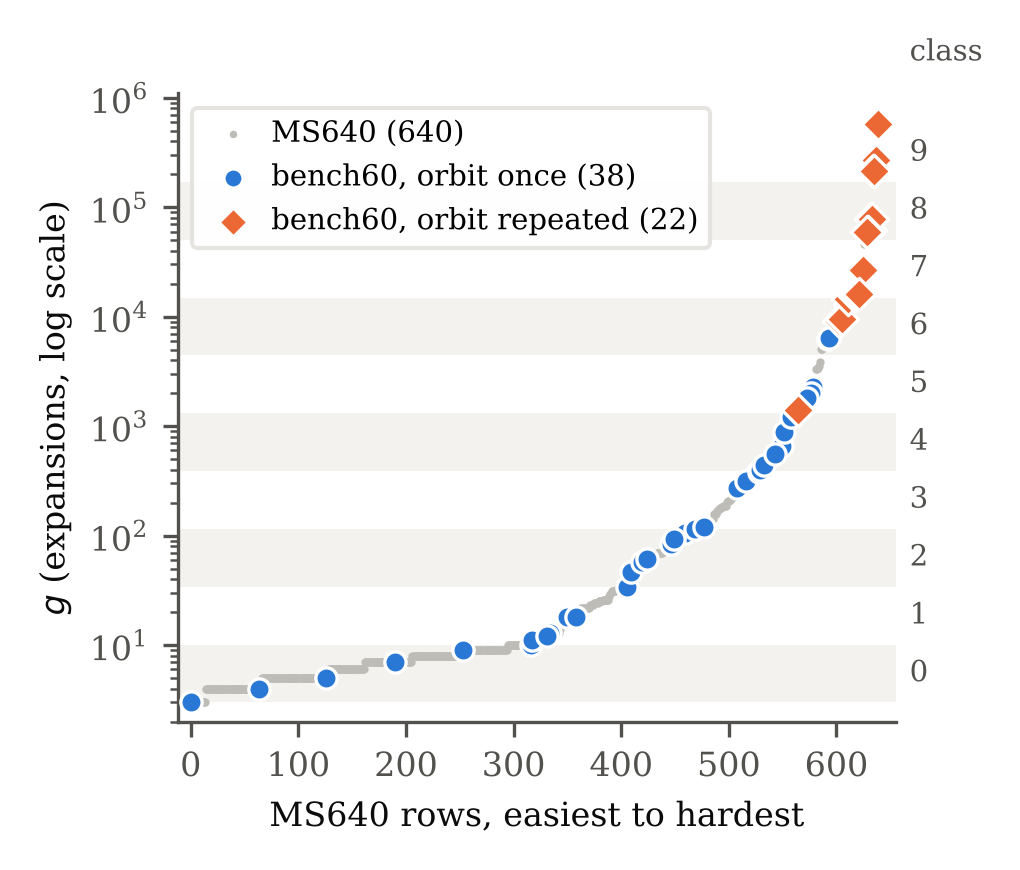
\includegraphics[width=0.49\textwidth]{figures/bench60_g.png}\hfill
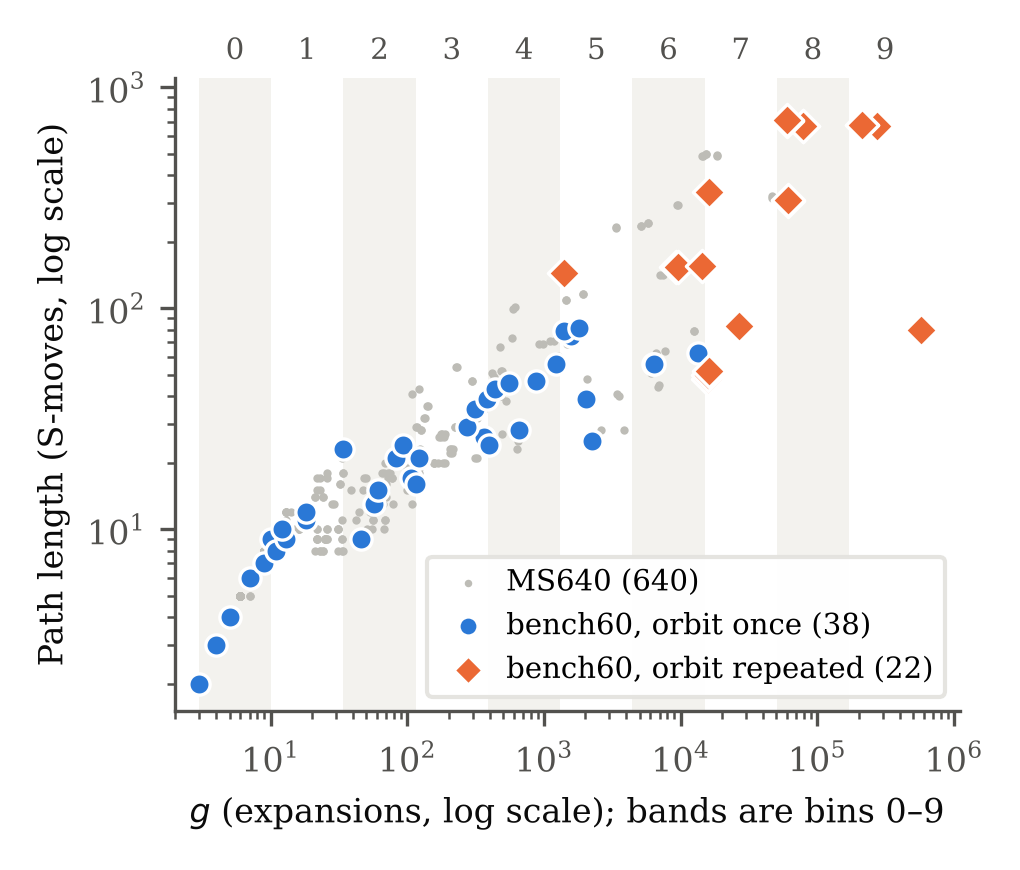
\includegraphics[width=0.49\textwidth]{figures/bench60_path.png}
\caption{bench60 inside MS640. Grey: all $640$ presentations; colour: the $60$ choices, six per difficulty class. Blue circles are choices whose
$\Aut(\F_2)$-orbit occurs once in bench60; diamonds are choices that share an orbit with another choice, which classes 7--9 force.
Left: $g$ against the rows sorted by $g$; the shaded bands are difficulty classes 0--9, each $3.37$ times the one below.
Right: the S-move length of a presentation against $g$.}
\label{fig:bench60}
\end{figure}

\subsection{ladder100}\label{app:ladder}

Each level of ladder100 (Definition~\ref{def:ladder}) contains $10$ presentations taken from AC19\_autmin and MS640;
Table~\ref{tab:ladder} gives the range of $g$ of each level. Here $g>10^7$ indicates that LENGTH fails within $10^7$
expansions, and $g_S$ denotes the number of expansions that $\SMK$ requires. At levels $1$--$6$ the presentations are
spread over the range of $g$ of the level, and at level $9$ over the range of $g_S$. Level $7$ takes the presentations
with the largest $g_S$, and level $8$ those with the largest $g$. Level $10$ consists of the presentations on which
$\SMK$ also fails within $10^7$ expansions.

Every presentation of ladder100 is AC-trivial. Those taken from MS640 are solved by LENGTH. For a presentation of
AC19\_autmin, the corresponding presentation of the extended AC19 data set is solved, and its S-moves are carried over to
the $\Aut(\F_2)$-minimal form.

\begin{table}[ht]
\centering
\begin{tabular}{rlrrrr}
\toprule
level & $g$ & from MS640 & mean $\lambda$ & mean $g$ & mean $g_S$\\
\midrule
1 & $<10^3$ & $5$ & $15.3$ & $214$ & $101$\\
2 & $10^3$--$10^4$ & $5$ & $19.9$ & $3{,}983$ & $707$\\
3 & $10^4$--$10^{4.5}$ & $5$ & $21.1$ & $17{,}612$ & $7{,}646$\\
4 & $10^{4.5}$--$10^5$ & $5$ & $21.5$ & $56{,}183$ & $9{,}780$\\
5 & $10^5$--$10^{5.5}$ & $4$ & $22.5$ & $235{,}756$ & $13{,}312$\\
6 & $10^{5.5}$--$10^6$ & $2$ & $19.4$ & $588{,}638$ & $4{,}693$\\
7 & $10^6$--$3\cdot10^6$ & $0$ & $20.2$ & $1{,}875{,}962$ & $424{,}977$\\
8 & $3\cdot10^6$--$10^7$ & $0$ & $18.8$ & $5{,}022{,}975$ & $113{,}309$\\
9 & $>10^7$ & $0$ & $21.0$ & -- & $340{,}650$\\
10$^{*}$ & $>10^7$ & $0$ & $18.3$ & -- & --\\
\bottomrule
\end{tabular}

\smallskip
{\small $^{*}$Only $9$ presentations fail for $\SMK$, so the tenth, \texttt{ac19\_12445}, is the next hardest one for
$\SMK$ from level $9$: it needs $1{,}297{,}772$ expansions.}
\caption{The levels of ladder100: the range of $g$, the number of the $10$ presentations taken from MS640 (the rest
are from AC19\_autmin), and the means of the starting total length $\lambda$, of $g$ and of $g_S$.}
\label{tab:ladder}
\end{table}

\subsection{Time per unit}\label{app:time}

An expansion performs different work in each method. LENGTH and $\SMK$ differ only in the priority they compute; the
hybrid additionally constructs the Nielsen images and runs the finishing checks; and a change of variables constructs
images of the state in place of S-move children. Equal budgets in units therefore constitute a fair comparison only
if a unit costs approximately the same in each method. To quantify the difference, one expansion of each method is
timed on the same states. For each test state, each method starts a fresh search, so that the heap holds only that
state, and performs one expansion: it removes the state, generates all of its children, discards those already
discovered, computes the priorities of the remainder and pushes them onto the heap. The test states are drawn at random
from the states that LENGTH and $\SMK$ expanded on MS640 with a budget of $10^4$ units, up to $60$ per range of total
length $\lambda$, and every method is timed on the same states. All methods run in pure Python (one core, Intel Xeon
$2.1$ GHz, best of five runs).
\begin{center}
\small
\begin{tabular}{lrrrrr}
\toprule
$\lambda$ & states & LENGTH & $\SMK$ & hybrid & CoV\\
\midrule
$\le10$ & $46$ & $0.12$ & $0.14$ & $0.28$ & $0.25$\\
$11$--$15$ & $60$ & $0.85$ & $1.05$ & $1.37$ & $3.24$\\
$16$--$20$ & $60$ & $1.61$ & $2.00$ & $3.03$ & $6.05$\\
$21$--$25$ & $60$ & $2.99$ & $3.41$ & $10.08$ & $11.23$\\
$\ge26$ & $60$ & $4.66$ & $6.00$ & $6.85$ & $16.47$\\
\midrule
mean & & $2.04$ & $2.52$ & $4.32$ & $7.45$\\
relative to LENGTH & & $1$ & $1.23$ & $2.11$ & $3.64$\\
\bottomrule
\end{tabular}

\smallskip
\footnotesize Time of one pop in ms, averaged over the states of the row. The mean row averages the five rows; the last row divides it by the LENGTH mean.
\end{center}
For example, one expansion of $\mathrm{AK}(3)$ ($\lambda=13$) takes $0.69$ ms for LENGTH, $0.87$ ms for $\SMK$,
$1.17$ ms for the hybrid and $2.61$ ms for the change of variables. A longer state has more children, so its expansion
costs more. An expansion of $\SMK$ differs from one of LENGTH only in its priority and costs $1.1$--$1.3$ times as much.
An expansion of the hybrid also constructs the four Nielsen images and runs the finishing checks, and costs $1.5$--$3.4$
times as much; its remaining units are single moves and cost less. Constructing the change-of-variables images of a
state costs $3.5$--$3.8$ expansions of LENGTH for $\lambda>10$. A unit of each method thus costs within a small factor
of one expansion of LENGTH, and equal budgets in units are comparable up to that factor.
